\documentclass[border=2pt]{standalone}
% Shared TikZ styles for the System One vs LLM diagrams (compiled as standalone PDFs).
\usepackage[T1]{fontenc}
\usepackage{lmodern}
\usepackage[english]{babel}
\usepackage{tikz}
\usetikzlibrary{shapes.geometric,positioning,fit,arrows.meta,calc,backgrounds}
\definecolor{ioFill}{HTML}{F1F0EC}\definecolor{ioLine}{HTML}{52514E}
\definecolor{modFill}{HTML}{E8F1FB}\definecolor{modLine}{HTML}{2A78D6}
\definecolor{decFill}{HTML}{ECE9F7}\definecolor{decLine}{HTML}{4A3AA7}
\definecolor{postFill}{HTML}{FFF6E0}\definecolor{postLine}{HTML}{EDA100}
\definecolor{loopRed}{HTML}{E34948}\definecolor{clusterLine}{HTML}{9A9890}
\tikzset{
  every node/.style={font=\small, align=center},
  hyphens off/.style={},
  io/.style={trapezium, trapezium left angle=72, trapezium right angle=108, trapezium stretches body,
             draw=ioLine, fill=ioFill, thick, inner sep=3pt, minimum height=2.6em},
  model/.style={rectangle, draw=modLine, fill=modFill, very thick, inner sep=4pt, minimum height=2.6em, text width=#1},
  model/.default=3.6cm,
  post/.style={rectangle, draw=postLine, fill=postFill, very thick, inner sep=4pt, minimum height=2.2em, text width=3.6cm},
  decision/.style={diamond, aspect=1.9, draw=decLine, fill=decFill, very thick, inner sep=1pt},
  arrow/.style={-{Latex[length=2mm]}, thick, ioLine},
  loop/.style={-{Latex[length=2.4mm]}, line width=1.4pt, loopRed},
  cluster/.style={draw=clusterLine, dashed, rounded corners=3pt, inner sep=7pt, fill=white},
  clusterlabel/.style={font=\small\bfseries, text=ioLine},
}

\begin{document}
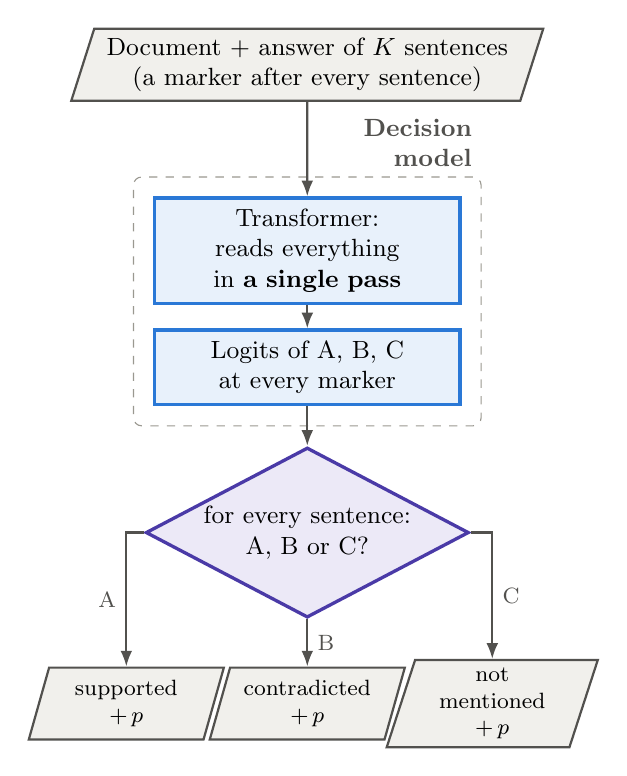
\begin{tikzpicture}[node distance=5mm]
  \node[io, text width=5.2cm] (in) {Document + answer of $K$ sentences\\(a marker after every sentence)};
  \node[model, below=12mm of in] (t) {Transformer: reads everything\\in \textbf{a single pass}};
  \node[model, below=3mm of t] (r) {Logits of A, B, C\\at every marker};
  \begin{scope}[on background layer]
    \node[cluster, fit=(t)(r), label={[clusterlabel,anchor=south east,align=right]north east:{Decision\\model}}] (c) {};
  \end{scope}
  \node[decision, below=5mm of r] (d) {for every sentence:\\A, B or C?};
  \node[io, below=6mm of d, font=\footnotesize, text width=1.75cm] (o2) {contradicted\\$+\,p$};
  \node[io, left=0.5mm of o2, font=\footnotesize, text width=1.75cm] (o1) {supported\\$+\,p$};
  \node[io, right=0.5mm of o2, font=\footnotesize, text width=1.75cm] (o3) {not\\mentioned\\$+\,p$};
  \draw[arrow] (in) -- (t);
  \draw[arrow] (t) -- (r);
  \draw[arrow] (r) -- (d);
  \draw[arrow] (d.west) -| node[pos=0.75, left, font=\footnotesize] {A} (o1.north);
  \draw[arrow] (d.south) -- node[right, font=\footnotesize] {B} (o2.north);
  \draw[arrow] (d.east) -| node[pos=0.75, right, font=\footnotesize] {C} (o3.north);
\end{tikzpicture}
\end{document}
